\documentclass{article}
\usepackage[utf8]{inputenc}
\usepackage[T1]{fontenc}
\usepackage{graphicx}
\usepackage{hyperref}
\usepackage{geometry}
\geometry{margin=1in}

\title{AMI  619 A M I}
\date{Encyclopaedia Britannica (1771)}

\begin{document}
\maketitle

\section*{Historical source}
\textbf{Entry ID:} \texttt{entry-ami-619-a-m-i-560} \\
\textbf{Volume ID:} 191253801 \\
\textbf{Character Count:} 1622

\subsection*{Extracted Text}
Amothy- gular, feminquinquifed, and perfilient: The \_courillo\_ is monospensioning. the border infiquorites are found in the \_famina confitt\_ of two slender filaments appreciated; the authors are simple and rounded. The \_pilliflora has a four-clet german i fylvia\_, the fate of the flaminis a figmatts two acurs No \_corella :\_ The \_feels form; globos, and shorter than the colyx – There is only one known facec.

This plant is a native of Siberia, from whence the feeds were fet to the imperial garden at Peterburgh, and these brought to Russian. It is an amazing plant, with an upright folk, which rifles about a foot high. Towards the top it puts forth was on three fossil line related branches, garnished with small del leaves, lived on their edges, of a very dark green colour. The flowers appear in June or July, and are produced in final until all the extremities of the branches. They are of a fine blue colour, as are also the upper part of the branches, and the leaves immediately under the unshl, for that dry makes a fine appearance.

\_Culture.\_ The feeds of the amethyaites should be flown in autumn as they set up to remain a whole year in the ground if kept till the living. When the plants come up, nothing else is necefitary than to keep them clear of weeds, and to thin them where they are too clede. They ought to be down where they are to re main, as they do not thrive when transparent.

AMPHYSTIVE is applied, in antiguity, to a kind of purple garment dyed of the bus of amethyft. In this fenêm amethyfilne differed from \_Tyrian\_ as well as from \_breathine\_ purple, being a kind of medium between both.



\section*{Source record}
\begin{itemize}
\item \textbf{Dataset:} \texttt{NationalLibraryOfScotland/encyclopaedia\_britannica\_illustrated}
\item \textbf{Dataset Revision:} \texttt{309f765b1ecc83e0a7f7762e44b4a927a7555443}
\item \textbf{Page ID:} \texttt{britannica:309f765b1ecc83e0a7f7762e44b4a927a7555443:train:560} \\
  \textbf{Filename:} \texttt{page-0560-c458f594fc79.jpg} \\
  \textbf{Row Index:} 560 \\
  \textbf{SHA256:} \texttt{c458f594fc79392e...}
\end{itemize}

\begin{figure}[h]
\centering
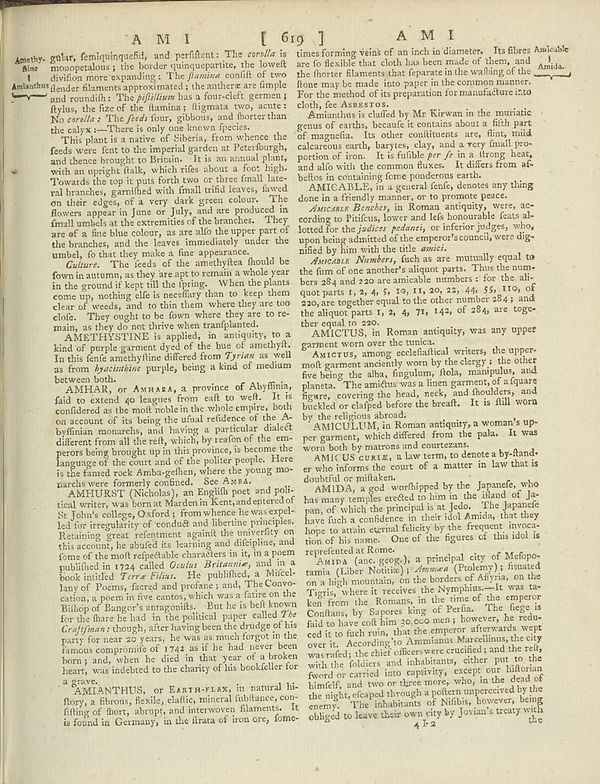
\includegraphics[width=0.85\textwidth]{../scans/page-0560-c458f594fc79.jpg}
\caption*{Source scan: \texttt{page-0560-c458f594fc79.jpg}}
\end{figure}

\end{document}
